\documentclass[utf8, a4paper, 14pt, russian, oneside]{book}

% Размер шрифта
\usepackage[14pt]{extsizes}

% Кодировка
\usepackage[T2A]{fontenc}
\usepackage[utf8]{inputenc}
\usepackage[main=russian, english]{babel}

\usepackage{fontspec}
\setmainfont{Times New Roman}
\usepackage{sectsty}
\sectionfont{\large}
\subsectionfont{\large}

% Параметры страницы
\usepackage[left=3cm, right=1cm, top=2cm, bottom=2cm]{geometry}
\pagestyle{plain}
\linespread{1.1} % Межстрочный интервал

% Пакеты для работы с математикой
\usepackage{amsmath}
\usepackage{amsfonts}
\usepackage{amssymb}

% Вставка изображений
\usepackage{graphicx}

% Пакет для работы с таблицами
\usepackage{tabularx}
\usepackage{booktabs}
\usepackage{longtable}

% Для больших множеств
\usepackage{mathtools}

% Для работы с рисунками
\usepackage{caption}

% Для создания графов в 3 блоке
\usepackage[all]{xy}

% Для специальных символов
\usepackage{textcomp}

% Для гиперссылок
\usepackage{hyperref}

% Для таблиц
\usepackage{multirow}

\usepackage{upgreek}

\usepackage{array}
\newcommand{\mysec}[1]{
{\centering\section*{\hyperlink{toc}{#1}}}
\addcontentsline{toc}{section}{#1}
}

\newcommand{\mysubsec}[1]{
{\centering\subsection*{\hyperlink{toc}{#1}}}
\addcontentsline{toc}{subsection}{#1}
}

\newcommand{\Db}{
    \ensuremath{
        D_{\text{в}}
    }
}

\newcommand{\xb}{
    \ensuremath{
        x_{\text{в}}
    }
}

\newcommand{\yb}{
    \ensuremath{
        y_{\text{в}}
    }
}

\newcommand{\zb}{
    \ensuremath{
        z_{\text{в}}
    }
}

\newcommand{\yx}{
    \ensuremath{
        y_x
    }
}

\newcommand{\zx}{
    \ensuremath{
        z_x
    }
}

\newcommand{\cov}{
    \ensuremath{
        \mathit{cov}_{\text{в}}
    }
}

\renewcommand{\r}{
    \ensuremath{
        \mathit{r}_{\text{в}}
    }
}

\newcommand{\rang}{
    \ensuremath{
        \mathit{rang}
    }
}

\newcommand{\rhob}{
    \ensuremath{
        \rho_{\text{в}}
    }
}

\newcommand{\der}[2]{
    \ensuremath{
        \frac{\partial #1}{\partial #2}
    }
}

% Команды для настройки содержания
\renewcommand\contentsname{\center{Содержание}} % Вместо оглавления пишется содержание
\addto{\captionsenglish}{\renewcommand{\bibname}{References}}
\begin{document}

\thispagestyle{empty}
~\vspace{-2cm}\setlength{\parindent}{0cm}
\begin{center}
	
\includegraphics[scale=1.5]{../include/logo.png}\\[2pt]
	МИНОБРНАУКИ РОССИИ\\
	Федеральное государственное бюджетное образовательное учреждение\\
	высшего профессионального образования\\[5pt]
	\textbf{<<МИРЭА – Российский технологический университет>>}\\[5pt]
	\textbf{\large РТУ МИРЭА}\\[20pt]
	\hrule{}\mbox{}\\[1pt]
	\hrule{}\mbox{}\\[20pt]	
	Институт кибернетики \\ Кафедра <<Информационная безопасность>> (БК №252)\\[35pt]
	\textbf{Долгосрочное задание} \\
	по дисциплине: Математическая статистика
\end{center}
	\vspace{4in}
	Студент группы ККСО-01-19:  \qquad \qquad \qquad  \qquad     Колесников А.В.
\vspace{0.6in}
\begin{center}
Москва --- 2021
\end{center}
\newpage

\tableofcontents
\newpage

\mysec{Описание данных}
Среднее время круга в гонках Formula-1 c 1971 по 2020г в секундах. \footnote{http://ergast.com/mrd/db/}
\begin{table}[h!]
    \centering
    \begin{tabular}{|c|c|c|c|}
        \hline
        Год & Время & Год & Время \\ \hline
        1971 & 26,9 & 1996 & 22,5 \\ \hline
        1972 & 25,0 & 1997 & 24,7 \\ \hline
        1973 & 23,4 & 1998 & 16,9 \\ \hline
        1974 & 23,2 & 1999 & 23,1 \\ \hline
        1975 & 23,8 & 2000 & 25,1 \\ \hline
        1976 & 23,6 & 2001 & 24,5 \\ \hline
        1977 & 22,6 & 2002 & 24,2 \\ \hline
        1978 & 24,9 & 2003 & 24,0 \\ \hline
        1979 & 25,3 & 2004 & 23,2 \\ \hline
        1980 & 25,3 & 2005 & 26,3 \\ \hline
        1981 & 23,0 & 2006 & 25,7 \\ \hline
        1982 & 23,2 & 2007 & 24,3 \\ \hline
        1983 & 24,5 & 2008 & 22,7 \\ \hline
        1984 & 23,7 & 2009 & 23,9 \\ \hline
        1985 & 24,1 & 2010 & 24,8 \\ \hline
        1986 & 26,0 & 2011 & 26,4 \\ \hline
        1987 & 24,9 & 2012 & 26,2 \\ \hline
        1988 & 20,9 & 2013 & 26,3 \\ \hline
        1989 & 24,5 & 2014 & 24,2 \\ \hline
        1990 & 24,9 & 2015 & 24,1 \\ \hline
        1991 & 24,0 & 2016 & 31,7 \\ \hline
        1992 & 23,8 & 2017 & 32,0 \\ \hline
        1993 & 23,3 & 2018 & 22,6 \\ \hline
        1994 & 23,4 & 2019 & 22,8 \\ \hline
        1995 & 33,9 & 2020 & 22,6 \\ \hline
    \end{tabular}
\end{table}
\newpage

\mysec{Простейшие способы обработки статистических данных}
Порядковая статистика:
\begin{table}[h!]
    \centering
    \begin{tabular}{|c|c|c|c|c|c|c|c|c|c|}
        \hline
        20,9 & 20,9 & 22,5 & 22,6 & 22,6 & 22,6 & 22,7 & 22,8 & 23,0 & 23,1\\
        \hline
        23,2 & 23,2 & 23,3 & 23,3 & 23,4 & 23,4 & 23,6 & 23,7 & 23,8 & 23,8\\
        \hline
        23,9 & 24,0 & 24,0 & 24,1 & 24,1 & 24,2 & 24,2 & 24,3 & 24,5 & 24,5\\
        \hline
        24,5 & 24,7 & 24,8 & 24,9 & 24,9 & 24,9 & 25,0 & 25,1 & 25,3 & 25,3\\
        \hline
        25,7 & 26,0 & 26,2 & 26,3 & 26,3 & 26,4 & 28,9 & 31,7 & 33,0 & 33,9\\
        \hline
    \end{tabular}
\end{table}

Вариации:
\begin{table}[h!]
    \centering
    \begin{tabular}{|c|c|c|c|c|c|c|c|c|c|}
        \hline
        20,9 & 22,5 & 22,6 & 22,7 & 22,8 & 23,0 & 23,1 & 23,2 & 23,3 & 23,4\\
        \hline
        23,6 & 23,7 & 23,8 & 23,9 & 24,0 & 24,1 & 24,2 & 24,3 & 24,5 & 24,7\\
        \hline
        24,8 & 24,9 & 25,0 & 25,1 & 25,3 & 25,7 & 26,0 & 26,2 & 26,3 & 26,4\\
        \hline
        28,9 & 31,7 & 33,0 & 33,9 & & & & & &\\
        \hline
    \end{tabular}
\end{table}

Мода -самые частые вариации: $M_1 = 22,6; M_2 = 24,5; M_3 = 24,9$. Вариации $x_i = 22,6$, $x_i=24,5$, $x_i = 24,9$ встречаются по 3 раза.

Медина - наблюдение, стоящее в середине порядковой выборки. Поскольку объём выборки чётное число ($n=50$), то медиану посчитаем по следующей формуле:
\begin{align*}
    m = \frac{x_{\tfrac{n}{2}} + x_{\tfrac{n}{2} + 1}}{2} = \frac{24,1 + 24,2}{2} = 24,15
\end{align*}

Построим вариационный ряд:
\begin{table}[h!]
    \begin{tabular}{|c|c|c|c|c|c|c|c|c|c|c|}
        \hline
        $x_i$ & 20,9 & 22,5 & 22,6 & 22,7 & 22,8 & 23,0 & 23,1 & 23,2 & 23,3 & 23,4 \\
        \hline
        $n_i$ & 2 & 1 & 3 & 1 & 1 & 1 & 1 & 2 & 2 & 2\\
        \hline
        $w_i$ & 0,04 & 0,02 & 0,06 & 0,02 & 0,02 & 0,02 & 0,02 & 0,04 & 0,04 & 0,04 \\
        \hline
    \end{tabular}
\end{table}
\begin{table}[h!]
    \begin{tabular}{|c|c|c|c|c|c|c|c|c|c|c|}
        \hline
        $x_i$ & 23,6 & 23,7 & 23,8 & 23,9 & 24,0 & 24,1 & 24,2 & 24,3 & 24,5 & 24,7 \\
        \hline
        $n_i$ & 1 & 1 & 2 & 1 & 2 & 2 & 2 & 1 & 3 & 1 \\
        \hline
        $w_i$ & 0,02 & 0,02 & 0,04 & 0,02 & 0,04 & 0,04 & 0,04 & 0,02 & 0,06 & 0,02 \\
        \hline
    \end{tabular}
\end{table}
\newpage
\begin{table}[h!]
    \begin{tabular}{|c|c|c|c|c|c|c|c|c|c|c|}
        \hline
        $x_i$ & 24,8 & 24,9 & 25,0 & 25,1 & 25,3 & 25,7 & 26,0 & 26,2 & 26,3 & 26,4 \\
        \hline
        $n_i$ & 1 & 3 & 1 & 1 & 2 & 1 & 1 & 1 & 2 & 1 \\
        \hline
        $w_i$ & 0,02 & 0,06 & 0,02 & 0,02 & 0,04 & 0,02 & 0,02 & 0,02 & 0,04 & 0,02 \\
        \hline
    \end{tabular}
\end{table}
\begin{table}[h!]
    \begin{tabular}{|c|c|c|c|c|c|c|c|c|c|c|}
        \hline
        $x_i$ & 28,9 & 31,7 & 33,0 & 33,9\\
        \hline
        $n_i$ & 1 & 1 & 1 & 1 \\
        \hline
        $w_i$ & 0,02 & 0,02 & 0,02 & 0,02 \\
        \hline
    \end{tabular}
\end{table}

$x_i$ - значения, попавшие в выборку.\\
$n_i$ - частота вариации $x_i$.\\
$w_i$ - относительная частота вариации $x_i$.

{
\centering
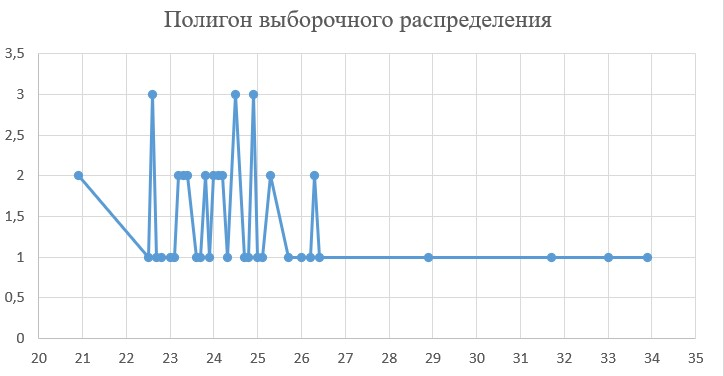
\includegraphics[scale=0.85]{img/poligon.jpg}
}

Пусть $k$ - число вариаций.

Выборочное среднее - среднее арифметическое значений выборки:
\begin{align*}
    \overline{x}_B = \sum\limits_{i=1}^{k}x_i w_i = 20,9 \cdot 0,04 + 22,5 \cdot 0,02 + \ldots + 33,9 \cdot 0,02 = 24,68.
\end{align*}

Выборочная дисперсия - мера разброса значений выборки относительно ее среднего:
\begin{align*}
    D_B(x) = \sum\limits_{i=1}^{k}x_i^2w_i - (\overline{x}_B)^2 = 20,9^2 \cdot 0,04 + \ldots + 33,9^2 \cdot 0,02 - (24,64)^2 = 6,26.
\end{align*}

Выборочное среднеквадратическое отклонение:
\begin{align*}
    \sigma_B(x) = \sqrt{{D_B(x)}} = \sqrt{6,26} = 2,5
\end{align*}
\newpage

\mysec{Доверительные интервалы}
Доверительный интервал математического ожидания при известном $\sigma_B(x)$:
\begin{align*}
    a \in \left( \overline{x}_B - t_{\gamma}\frac{\sigma}{\sqrt{n}}; \quad \overline{x}_B + t_{\gamma}\frac{\sigma}{\sqrt{n}} \right).
\end{align*}

Величина $t_{\gamma}$ находится из следующего равенства:
\begin{align*}
    2\Phi(t_\gamma) = \gamma,\  \text{где}\  \gamma\ \text{-доверительная вероятность.}
\end{align*}

Если $\gamma = 0,95,$ то $\Phi(t_\gamma) = 0,475$, а $t_\gamma = 1,96$.\\
Если $\gamma = 0,99,$ то $\Phi(t_\gamma) = 0,495$, а $t_\gamma = 2,86$.

Поскольку $\sigma = 3.1$, то при доверительной вероятности $\gamma = 0,95$ верно следующее:
\begin{align*}
    a \in \Big(24,68 - 1,96\cdot \frac{2,5}{\sqrt{50}};\  & 24,68 + 1,96\cdot \frac{2,5}{\sqrt{50}}\Big), \\
    a \in ( 23,98;\  & 25,37 ).
\end{align*}

При доверительной вероятности $\gamma=0,99$ верно:
\begin{align*}
    a \in \Big(24,68 - 2,86\cdot \frac{2,5}{\sqrt{50}};\  & 24,68 + 2,86\cdot \frac{2,5}{\sqrt{50}}\Big), \\
    a \in ( 23,67;\  & 25,69 ).
\end{align*}

Доверительный интервал математического ожидания при неизвестном $\sigma_B(x)$:
Так как $\sigma_B(x)$ неизвестно, то вычислим исправленную выборочную дисперсию:
\begin{align*}
    s^2 = \frac{n}{n-1}D_B(x) &= \frac{50}{49} \cdot 6,25 = 6,38 \\
    s = \sqrt{s^2} &= \sqrt{6,38} = 2,52 \\ 
    a \in \Big( \overline{x}_B - t_\gamma\frac{s}{\sqrt{n}};\  & \overline{x}_B + t_\gamma\frac{s}{\sqrt{n}} \Big)
\end{align*}

В данном случае $t_\gamma$ берётся из таблицы Стьюдента. $df = 50 - 1 = 49$.\\
Для $\gamma = 0,95: t_{0,95} = 2,022.$\\
Для $\gamma = 0,99: t_{0,99} = 2,680.$\\

При доверительной вероятности $\gamma=0,95$ верно:
\begin{align*}
    a \in \Big( 24,68 - 2,022 \cdot \frac{2,52}{\sqrt{50}};\  & 24,68 + 2,022 \cdot \frac{2,52}{\sqrt{50}} \Big)\\
    a \in ( 23,96;\  & 25,4).
\end{align*}

При доверительной вероятности $\gamma=0,99$ верно:
\begin{align*}
    a \in \Big( 24,68 - 2,680 \cdot \frac{2,52}{\sqrt{50}};\  & 24,68 + 2,680 \cdot \frac{2,52}{\sqrt{50}} \Big)\\
    a \in ( 23,72;\ & 25,63).
\end{align*}

Доверительный интервал дисперсии при неизвестном математическом ожидании:
\begin{align*}
    \sigma^2 \in \Bigg( \frac{(n-1)s^2}{\chi^2_{\tfrac{1+\gamma}{2},n-1}};\ & \frac{(n-1)s^2}{\chi^2_{\tfrac{1-\gamma}{2},n-1}} \Bigg)\\
    \frac{1-\gamma_1}{2} = \frac{1 - 0,95}{2} = 0,025; \quad& \frac{1+\gamma_1}{2} = \frac{1+0,95}{2} = 0,975\\
    \frac{1-\gamma_2}{2} = \frac{1 - 0,99}{2} = 0,005; \quad& \frac{1+\gamma_2}{2} = \frac{1+0,99}{2} = 0,995\\
    \chi^2_{0,975;49} = 70,22 \qquad& \chi^2_{0,025;49} = 31,55 \\
    \chi^2_{0,995;49} = 78,23 \qquad& \chi^2_{0,005;49} = 27,25
\end{align*}

При доверительной вероятности $\gamma=0,95$ верно:
\begin{align*}
    \sigma^2 \in \Big( \frac{49 \cdot 6,38}{70,22};\  & \frac{49 \cdot 6,38}{31,55} \Big)\\
    \sigma^2 \in (4,45;\  & 9,91)\\
    \sigma \in (2,11;\  & 3,15)
\end{align*}

При доверительной вероятности $\gamma=0,99$ верно:
\begin{align*}
    \sigma^2 \in \Big( \frac{49 \cdot 6,38}{78,23};\  & \frac{49 \cdot 6,38}{27,25} \Big)\\
    \sigma^2 \in (3.99;\  & 11,47)\\
    \sigma \in (1.99;\  & 3,37)
\end{align*}

\newpage

\mysec{Интервальный вариационный ряд и его характеристики}
Имеется 50 значений от 20,9 до 33,9. Пусть левая граница значения будет равна 20. Получаем отрезок [16;37,9].
Пусть длина интервала $h=2$.
Если значене $x_i$ попадает на границу интервалов и $x_i$ является нечётным числом, то большую часть относим к левому интервалу, в противном
случае делим попалам.
\begin{table}[h!]
    \centering
    \begin{tabular}{|c|c|c|c|c|c|c|c|}
        \hline
        $I_i$ & [20;22] & [22;24] & [24;26] & [26;28] & [28;30] & [30;32] & [32;34]\\
        \hline
        $n_i$ & 2 & 20 & 20 & 4 & 1 & 1 & 2 \\
        \hline
        $w_i$ & 0,04 & 0,4 & 0,4 & 0,08 & 0,02 & 0,02 & 0,04 \\
        \hline
    \end{tabular}
\end{table}

$I_i$ - интервал с номером $i$;\\
$n_i$ - количество вариаций $x_i$, попавших в интервал $I_i$;\\
$w_i$ - относительная частота.

% Гистограмма выборки
\begin{center}
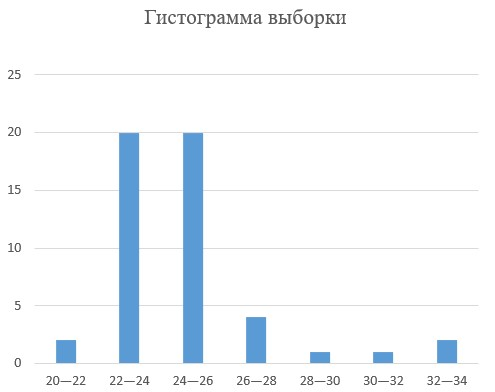
\includegraphics[scale=0.95]{img/gisto_choice.jpg}
\end{center}

Для того, чтобы определить к какой совокупности относится выборка проведём статистическую проверку.
\newpage

\mysubsec{Числовые характеристики интервального ряда}
\begin{table}[h!]
    \centering
    \begin{tabular}{|c|c|c|c|c|c|c|c|}
        \hline
        $x_i$ & 21 & 23 & 25 & 27 & 29 & 31 & 33\\
        \hline
        $n_i$ & 2 & 20 & 20 & 4 & 1 & 1 & 2 \\
        \hline
        $w_i$ & 0,04 & 0,4 & 0,4 & 0,08 & 0,02 & 0,02 & 0,04 \\
        \hline
    \end{tabular}
\end{table}

Выборочное среднее интервального ряда:
\begin{align*}
    \overline{x}_B^* = 21 \cdot 0,04 + 23 \cdot 0,4 + \ldots + 33 \cdot 0,04 = 24,72.
\end{align*}

Выборочная дисперсия интервального ряда:
\begin{align*}
    D_B*(x) = 21^2 \cdot 0,04 + 23^2 \cdot 0,4 + \ldots + 33^2 \cdot 0,04 - (24,72)^2 = 6,08
\end{align*}

Выборочное среднеквадратическое отклонение интервального ряда:
\begin{align*}
    \sigma_B^*(x) = \sqrt{D_B^*(x)} = 2,47
\end{align*}

Функция распределения определяется вероятностью того, что случайно выбранное значение из выборки окажется меньше аргумента функции.

Выборочная функция распределения интервального ряда:
\begin{align*}
    F_n^* =
    \begin{cases}
        0   ,&\ x \leq 21, \\
        0,04,&\  21 < x \leq 23, \\
        0,44,&\  23 < x \leq 25, \\
        0,84,&\  25 < x \leq 27, \\
        0,92,&\  27 < x \leq 29, \\
        0,94,&\  29 < x \leq 31, \\
        0,96,&\  31 < x \leq 33, \\
        1   ,&\  x > 33.
    \end{cases}
\end{align*}
\newpage

\mysec{Проверка на нормальный закон распределения}
Предположим, что данная выборка имеет нормальный закон распределения.

Обозначим $m_i$ - выровненную по нормальному закону частоту. Найдём её по следующей формуле:
\begin{align*}
    m_i = p_i \cdot n,
\end{align*}
где $p_i = p(\alpha < x < \beta) = \Phi(\tfrac{\beta - \overline{x}_B^*}{\sigma_B^*(x)}) - \Phi(\tfrac{\alpha - \overline{x}_B^*}{\sigma_B^*(x)})$, где
$\alpha$ и $\beta$ - границы интервала, $\overline{x}_B^*$ - выборочное среднее интервального ряда, $\sigma_B^*(x)$ - среднеквадратическое отклонение.

% TODO: Сделать вычисления до 3-х знаков после запятой

Выпишем значения функции Лапласа для каждой границы интервалов. Напомним, что $\overline{x}_B^* = 24,72$, $\sigma_B^*(x) = 2,47$.
\begin{align*}
    \Phi \left( \frac{20 - 24,72}{2,47} \right) &= -\Phi(1,91) = -0,47,\\
    \Phi \left( \frac{22 - 24,72}{2,47} \right) &= -\Phi(1,10) = -0,36,\\
    \Phi \left( \frac{24 - 24,72}{2,47} \right) &= -\Phi(0,29) = -0,11,\\
    \Phi \left( \frac{26 - 24,72}{2,47} \right) &=  \Phi(0,52) =  0,20,\\
    \Phi \left( \frac{28 - 24,72}{2,47} \right) &=  \Phi(1,33) =  0,41,\\
    \Phi \left( \frac{30 - 24,72}{2,47} \right) &=  \Phi(2,14) =  0,48,\\
    \Phi \left( \frac{32 - 24,72}{2,47} \right) &=  \Phi(2,95) =  0,49,\\
    \Phi \left( \frac{34 - 24,72}{2,47} \right) &=  \Phi(3,76) =  0,49.
\end{align*}

Получим, следующую таблицу значений:
\begin{table}[h!]
    \centering
    \begin{tabular}{|c|c|c|c|c|c|c|c|c|}
        \hline
        $\alpha_i$  & 20 & 22 & 24 & 26 & 28 & 30 & 32 & 34\\
        \hline
        $\Phi(\tfrac{\alpha_i - \overline{x}_B^*}{\sigma_B^*(x)})$ & -0,47 & -0,36 & -0,11 & 0,20 & 0,41 & 0,48 & 0,49 & 0,49\\
        \hline
    \end{tabular}
\end{table}

Для каждого интервала вычислим $p_i$:
\begin{align*}
    p_1 &= p(20 < x < 22) = -0,36 - ( -0,47 ) = 0,11, \\
    p_2 &= p(22 < x < 24) = -0,11 - ( -0,36 ) = 0,25, \\
    p_3 &= p(24 < x < 26) =  0,20 - ( -0,11 ) = 0,31, \\
    p_4 &= p(20 < x < 28) =  0,41 - (  0,20 ) = 0,21, \\
    p_5 &= p(28 < x < 30) =  0,48 - (  0,41 ) = 0,09, \\
    p_6 &= p(30 < x < 32) =  0,49 - (  0,48 ) = 0,01, \\
    p_7 &= p(32 < x < 34) =  0,49 - (  0,49 ) = 0. \\
\end{align*}

Получим, следующую таблицу значений:
\begin{table}[h!]
    \centering
    \begin{tabular}{|c|c|c|c|c|c|c|c|c|}
        \hline
        $p_1$ & $p_2$ &$p_3$ &$p_4$ &$p_5$ &$p_6$ &$p_7$ \\
        \hline
        0,11 & 0,25 & 0,31 & 0,31 & 0,09 & 0,01 & 0 \\
        \hline
    \end{tabular}
\end{table}

\newpage

\mysubsec{Выравние частот по нормальному закону}
\newpage

\mysubsec{Критерий $\chi^2$}
\newpage

\mysubsec{Нахождение уровня значимости}
\newpage

\mysubsec{Критерий Колмогорова}
\newpage

\mysec{Проверка на равномерное распределение}
\newpage

\mysubsec{Выравнивание частот по равномерному закону}
\newpage

\mysubsec{Критерий $\chi^2$}
\newpage

\mysubsec{Нахождение уровня значимости}
\newpage

\mysubsec{Критерий Колмогорова}
\newpage

\mysec{Вычисление выборочного коэффициента асимметрии и эксцесса}
\newpage

\mysec{Вывод}

\end{document}